\PassOptionsToPackage{unicode=true}{hyperref} % options for packages loaded elsewhere
\PassOptionsToPackage{hyphens}{url}
%
\documentclass[a4paper,twoside,11pt,chapterprefix=false,bibliography=totocnumbered,listof=flat]{scrbook}
\usepackage{lmodern}
\usepackage{amssymb,amsmath}
\usepackage{ifxetex,ifluatex}
\usepackage{fixltx2e} % provides \textsubscript
\ifnum 0\ifxetex 1\fi\ifluatex 1\fi=0 % if pdftex
  \usepackage[T1]{fontenc}
  \usepackage[utf8]{inputenc}
  \usepackage{textcomp} % provides euro and other symbols
\else % if luatex or xelatex
  \usepackage{unicode-math}
  \defaultfontfeatures{Ligatures=TeX,Scale=MatchLowercase}
\fi
% use upquote if available, for straight quotes in verbatim environments
\IfFileExists{upquote.sty}{\usepackage{upquote}}{}
% use microtype if available
\IfFileExists{microtype.sty}{%
\usepackage[]{microtype}
\UseMicrotypeSet[protrusion]{basicmath} % disable protrusion for tt fonts
}{}
\IfFileExists{parskip.sty}{%
\usepackage{parskip}
}{% else
\setlength{\parindent}{0pt}
\setlength{\parskip}{6pt plus 2pt minus 1pt}
}
\usepackage{hyperref}
\hypersetup{
            pdftitle={Sintassi Italiana 2},
            pdfauthor={Marco Petolicchio},
            pdfborder={0 0 0},
            breaklinks=true}
\urlstyle{same}  % don't use monospace font for urls
\usepackage{longtable,booktabs}
% Fix footnotes in tables (requires footnote package)
\IfFileExists{footnote.sty}{\usepackage{footnote}\makesavenoteenv{longtable}}{}
\usepackage{graphicx,grffile}
\makeatletter
\def\maxwidth{\ifdim\Gin@nat@width>\linewidth\linewidth\else\Gin@nat@width\fi}
\def\maxheight{\ifdim\Gin@nat@height>\textheight\textheight\else\Gin@nat@height\fi}
\makeatother
% Scale images if necessary, so that they will not overflow the page
% margins by default, and it is still possible to overwrite the defaults
% using explicit options in \includegraphics[width, height, ...]{}
\setkeys{Gin}{width=\maxwidth,height=\maxheight,keepaspectratio}
\setlength{\emergencystretch}{3em}  % prevent overfull lines
\providecommand{\tightlist}{%
  \setlength{\itemsep}{0pt}\setlength{\parskip}{0pt}}
\setcounter{secnumdepth}{5}
% Redefines (sub)paragraphs to behave more like sections
\ifx\paragraph\undefined\else
\let\oldparagraph\paragraph
\renewcommand{\paragraph}[1]{\oldparagraph{#1}\mbox{}}
\fi
\ifx\subparagraph\undefined\else
\let\oldsubparagraph\subparagraph
\renewcommand{\subparagraph}[1]{\oldsubparagraph{#1}\mbox{}}
\fi

% set default figure placement to htbp
\makeatletter
\def\fps@figure{htbp}
\makeatother

\usepackage[a4paper,margin=4cm, bindingoffset=1cm, heightrounded, headsep=2em, footskip=11mm, vmarginratio=1:1]{geometry}
\makeatletter
\DeclareOldFontCommand{\rm}{\normalfont\rmfamily}{\mathrm}
\DeclareOldFontCommand{\sf}{\normalfont\sffamily}{\mathsf}
\DeclareOldFontCommand{\tt}{\normalfont\ttfamily}{\mathtt}
\DeclareOldFontCommand{\bf}{\normalfont\bfseries}{\mathbf}
\DeclareOldFontCommand{\it}{\normalfont\itshape}{\mathit}
\DeclareOldFontCommand{\sl}{\normalfont\slshape}{\@nomath\sl}
\DeclareOldFontCommand{\sc}{\normalfont\scshape}{\@nomath\sc}
\makeatother




\usepackage{fontspec}

\usepackage{ifluatex}

\usepackage{microtype}



\setmainfont[Numbers=Lowercase]{IBMPlexSerif}
\setsansfont[Numbers=Lowercase]{IBMPlexSans}
\setmonofont[Numbers=Lowercase]{IBMPlexMono}


\usepackage[italian]{babel}

\usepackage[all]{nowidow}

\usepackage[usenames, dvipsnames]{color}
\definecolor{upol-dGrey}{rgb}{0.36470588235,0.36862745098,0.37647058823}
\definecolor{upol-lGrey}{rgb}{0.8,0.8,0.8}
\definecolor{upol-brandBlue}{rgb}{0,0.43529411764,0.67843137254}


\usepackage{xcolor}
\usepackage{graphicx}
\definecolor{titlepagecolor}{cmyk}{1,.38,0,.15} %C100 M38 Y0 K15
\definecolor{namecolor}{cmyk}{0, 0, 0, .0980} 
\usepackage{textcase}


\usepackage{setspace}

\makeatletter\let\Title\@title\makeatother
%\makeatletter\let\Author\@author\makeatother



\usepackage{sectsty}
\allsectionsfont{\color{upol-dGrey}\sffamily}
\chapterfont{\color{upol-dGrey}\raggedleft\thispagestyle{empty}}





\usepackage{floatrow}
\floatsetup[table]{font=sf}
\floatsetup[figure]{font=sf}
\floatsetup[tikzpicture]{font=sf}

\usepackage[font={color=upol-dGrey}, labelfont={color=upol-dGrey}]{caption}



\makeatletter
\def\verbatim@font{\linespread{1}\footnotesize\ttfamily}
\makeatother



\makeatletter
\renewenvironment{figure}[1][\fps@figure]{
  \edef\@tempa{\noexpand\@float{figure}[#1]} 
  \@tempa
  \sffamily
}{
  \end@float
}
\renewenvironment{table}[1][\fps@table]{
  \edef\@tempa{\noexpand\@float{table}[#1]} 
  \@tempa
  \sffamily
  \footnotesize
}{
  \end@float
}
\makeatother

\usepackage{tabularx}
\usepackage{amsfonts}
\usepackage{booktabs}
\usepackage{siunitx}
\usepackage{fancyhdr}

\usepackage{lipsum, kantlipsum} % just for testing

\pagestyle{fancy}
\fancyhf{}
\fancyhead[LE,RO]{\thepage}
\fancyhead[RE]{\footnotesize\nouppercase{\leftmark}}
\fancyhead[LO]{\footnotesize\nouppercase{\rightmark}}
\setlength{\headheight}{14.5pt} % as requested by fan
\renewcommand{\headrulewidth}{0pt}

\renewcommand{\chaptermark}[1]{\markboth{\thechapter \ . \  #1}{}}
\renewcommand{\sectionmark}[1]{\markright{\thesection \ \ #1}{}}





%\setcounter{secnumdepth}{5}
%\setsecnumdepth{subsubsection}
%\maxtocdepth{subsubsection}


\setlength{\skip\footins}{3em}
\renewcommand\footnoterule{{\hrule height 0pt}} % a long blue line



\usepackage{colortbl}
\arrayrulecolor{gray}







\usepackage{booktabs}

\usepackage{pdfpages}






%Options: Sonny, Lenny, Glenn, Conny, Rejne, Bjarne, Bjornstrup
\usepackage[Bjornstrup]{fncychap}
%\renewcommand{\CNoV}{\raggedleft\sffamily\selectfont\HUGE}
  \ChNumVar{\Huge\sffamily\selectfont}
\renewcommand{\DOCH}{%
   \settowidth{\py}{\CNoV\thechapter}
  \addtolength{\py}{1em}      % Amount of space by which the
%                                % number is shifted right
   \fboxsep=0pt%
   \colorbox[gray]{.85}{\rule{0pt}{50pt}\parbox[b]{\textwidth}{\hfill}}%
   \kern-\py\raise20pt%
   \hbox{\color{gray}\CNoV\thechapter}\\%
}

\makeatletter
\renewcommand*{\@makechapterhead}[1]{%
  \vspace*{0\p@}%
  {\parindent \z@ \raggedright \normalfont
    \ifnum \c@secnumdepth >\m@ne
      \if@mainmatter%%%%% Fix for frontmatter, mainmatter, and backmatter 040920
        \DOCH
      \fi
    \fi
    \interlinepenalty\@M
    \if@mainmatter%%%%% Fix for frontmatter, mainmatter, and backmatter 060424
      \DOTI{#1}%
    \else%
      \DOTIS{#1}%
    \fi
  }}
% For the case \chapter*:
\renewcommand*{\@makeschapterhead}[1]{%
  \vspace*{10\p@}%
  {\parindent \z@ \raggedright
    \normalfont
    \interlinepenalty\@M
    \DOTIS{#1}
    \vskip 0\p@
  }}
\makeatother




\renewcommand*\chapterpagestyle{empty}




\usepackage{tikz,tikz-qtree}
\usepackage{subcaption}


\tikzstyle{every picture}+=[font=\sffamily]

\usepackage{listings}
\lstset{ %Formatting for code in appendix
	backgroundcolor = \color{gray},
	language=Python,
	basicstyle=\singlespacing\footnotesize\ttfamily\color{white},
	numbers=left,
	stepnumber=1,
	showstringspaces=true,
	tabsize=2,
	breaklines=true,
	breakatwhitespace=false,
	xleftmargin=3em,framexleftmargin=3em, numberstyle=\ttfamily,
}

\usepackage{datetime}

\let\oldmaketitle\maketitle
\AtBeginDocument{\let\maketitle\relax}




\usepackage{catchfilebetweentags}

\usepackage[autostyle]{csquotes}  
\usepackage{enumerate}


\makeatletter
\newcommand\HUGE{\@setfontsize\Huge{36}{48}} 
\makeatother

\usepackage{tikz}
\usepackage{pgfplots}


\usepackage{gb4e,cgloss}
\noautomath

\let\eachwordone=\it



\makeatletter\renewcommand*{\fps@figure}{!h}\makeatother

\frontmatter
\usepackage[]{natbib}
\bibliographystyle{apa}

\title{Sintassi Italiana 2}
\providecommand{\subtitle}[1]{}
\subtitle{Dispense per gli studenti del corso KRI/SYNT2}
\author{Marco Petolicchio}
\date{2019-02-18}

\begin{document}
\maketitle

\makeatletter
\begin{titlepage}
\color{namecolor}

\pagecolor{titlepagecolor}

\noindent
\makebox[0pt][l]{\rule{1.4\textwidth}{1pt}}
\par

\noindent
\textbf{\sffamily{Palacký University}} \textcolor{namecolor}{\sffamily{ Olomouc}}\par \vskip\baselineskip 

\noindent\sffamily{Dipartimento di Lingue Romanze, Facoltà di Filosofia} \par\vskip\baselineskip

\vspace{2em}

\begin{flushleft}

\noindent
{\HUGE \sf \@title  \par}\vskip\baselineskip

\noindent
{\Large \sf \@subtitle \par} \vskip\baselineskip
\end{flushleft}

\noindent
{\large{\sffamily\MakeTextUppercase{\@author}}\par} 
\vspace{4em}
\par \vskip\baselineskip
\vspace{3em}

 {\footnotesize   \ttfamily{draft : : \today   : :  \currenttime} \par}

\color{black}

\end{titlepage}
\makeatother
\nopagecolor% Use this to restore the color pages to white
\pagecolor{white}

{
\setcounter{tocdepth}{1}
\tableofcontents
}
\listoftables
\listoffigures
\hypertarget{introduzione}{%
\chapter*{Introduzione}\label{introduzione}}
\addcontentsline{toc}{chapter}{Introduzione}

\begin{quote}
Se il mondo ha la struttura del linguaggio\\
e il linguaggio ha la forma della mente\\
la mente con i suoi pieni e i suoi vuoti\\
è niente o quasi e non ci rassicura.

E. Montale, \emph{La forma del mondo}, in \enquote{Diario del '71}
\end{quote}

\vfill

Questa dispensa nasce come materiale di studio per l'esame di Sintassi Italiana 2 per gli studenti triennali dell'Università Palacky di Olomouc, pensata in maniera specifica per studenti non madrelingua. Si fa riferimento a nozioni \emph{tradizionali} della linguistica e degli studi sintattici rimandando, laddove si è ritenuto più pertinente, a degli studi più recenti in maniera da poter stimolare ulteriormente lo studente.

Le abbreviazioni morfologiche e lo stile delle glosse interlineari aderiscono rispettivamente agli standard \emph{de facto} delle annotazioni di linguistica comparativa \citep[\href{http://www.oxfordhandbooks.com/view/10.1093/oxfordhb/9780199549368.001.0001/oxfordhb-9780199549368}{consultabile online}]{boeckxListOfAbbreviations} e dello stile delle glosse \emph{di Lipsia} \citep{leipzigGlossingRules}.

Nel testo si segue l'uso standard di definire i vari gradi di accettabilità di una frase attraverso le seguenti marche tipografiche:

\begin{itemize}
\tightlist
\item
  ( ) Grammaticale
\item
  (*) Agrammaticale
\item
  (?) Dubbia grammaticalità
\item
  (\#) Grammaticale dal punto di vista sintattico ma interpretazione semantica non coerente
\end{itemize}

Per qualsiasi informazione o suggerimento è possibile scrivere direttamente all'autore all'indirizzo \texttt{marco.petolicchio01@upol.cz} oppure aprire un issue direttamente sulla pagina del repository su \href{http://github.com/p-marco/sintassiIta2}{Github}.

Quest'opera è rilasciata con licenza Creative Commons BY 4.0. Il codice sorgente è disponibile all'indirizzo \texttt{http://github.com/p-marco/sintassiIta2} e le versioni del progetto sono rilasciate in DOI attraverso la piattaforma Zenodo (\url{DOI:10.5281/zenodo.2355707}).

\mainmatter

\part*{Parte I. \\\ Questioni preliminari}

\hypertarget{le-parti-del-discorso}{%
\chapter{Le parti del discorso}\label{le-parti-del-discorso}}

Le parole di una lingua vengono divise all'interno di categorie grammaticali. In italiano --una lingua flessiva come buona parte delle lingue indoeuropee \citep{graffiScalise2009}-- queste suddivisioni avvengono per criteri di natura sintattica, ovvero la posizione ed il ruolo delle parole all'interno della frase. Tradizionalmente possiamo riconoscere 9 diverse \textbf{parti del discorso} \citep{salvi2013}, tra cui possiamo operare una ulteriore suddivisione: quelle (parti) \emph{variabili} e quelle \emph{invariabili}.

\hypertarget{le-parti-variabili}{%
\section{Le parti variabili}\label{le-parti-variabili}}

In italiano si definiscono parti \textbf{variabili} del discorso quelle che hanno la possibilità di modificarsi sulla base di alcuni \emph{tratti} o \emph{categorie grammaticali} \citep[ Cap.9]{simone1995} come il Genere, il Numero, la Persona, il Caso, il Tempo, l'Aspetto, il Modo ecc..

\hypertarget{aggettivo}{%
\subsection{Aggettivo}\label{aggettivo}}

L'aggettivo è un \emph{modificatore} di altri elementi del discorso, soprattutto del sostantivo, con cui instaura un rapporto sintattico che si manifesta, nella maggior parte dei casi, nella concordanza grammaticale (\emph{Brutto stamani il tempo e ancora più pestifero il Tempo} \citep{montale-satura}, \emph{Le lasagne scaldate nel micro che da solo mi sento cattivo} \citep{fibra2017}).

Tradizionalmente possiamo suddividere la classe di aggettivi in due categorie:

\begin{itemize}
\tightlist
\item
  Determinativi:

  \begin{itemize}
  \tightlist
  \item
    Possessivi (\emph{mia, vostre, suo})
  \item
    Numerali:

    \begin{itemize}
    \tightlist
    \item
      Cardinali (\emph{due, trentatré})
    \item
      Ordinali (\emph{primo, quarantatreesimo})
    \end{itemize}
  \item
    Dimostrativi (\emph{questo, quello})
  \item
    Indefiniti (\emph{alcuni, tutti, nessuna})
  \item
    Interrogativi ed esclamativi (\emph{quale?, quanti?, quale gioia!, ma che onore!})
  \end{itemize}
\item
  Qualificativi (\emph{forte, grande, bello, rettangolare, goloso, verde, vecchio})
\end{itemize}

I determinativi esprimono alcune funzioni della referenza (per esempio il possesso), mentre i qualificativi esprimono dei caratteri quali il colore, la forma, l'aspetto, le qualità. Quella dei determinativi è una classe \emph{chiusa}, mentre quella dei qualificativi è una classe \emph{aperta} che prevede cioè la possibilità di espandersi in maniera indefinita.

\hypertarget{articolo}{%
\subsection{Articolo}\label{articolo}}

L'articolo è quella particella che si accompagna al nome o ad altre parti del discorso in funzione sostantivata. In italiano esso concorda nei tratti di Numero, Persona, Genere con il sostantivo di riferimento \citep{grandi2010}.
Le lingue del mondo non presentano tutte lo stesso comportamento nei riguardi della posizione e/o della presenza dell'articolo e possiamo trovare:

\begin{itemize}
\tightlist
\item
  Lingue senza articoli (\emph{ceco, slovacco})
\item
  Lingue con articoli

  \begin{itemize}
  \tightlist
  \item
    Proclitici (\emph{italiano, inglese})
  \item
    Enclitici (\emph{bulgaro, macedone})
  \end{itemize}
\end{itemize}

In una lingua come l'italiano, la presenza dell'articolo è lo \emph{standard}, ovvero non ha una funzione specifica mentre la sua assenza assume significato. Così, per esempio, in \textbf{italiano standard}\footnote{Alcune varietà di italiano, quali i dialetti settentrionali, hanno invece gli articoli in questi contesti \citep{loporcaro2009}.} i nomi propri escludono l'articolo (\emph{Marta va in città} vs.~\emph{*La Marta va in città}) così come è esclusa la possibilità di trovare l'articolo in combinazione con il possessivo nei nomi di famiglia (\emph{mio figlio si chiama Luigi} vs.~\emph{* Il mio figlio si chiama Luigi}).

\begin{table}[]
\begin{tabular}{@{}lrrrrrr@{}}
\toprule
      & \multicolumn{2}{c}{Definito} & \multicolumn{2}{c}{Indefinito} & \multicolumn{2}{c}{Partitivo} \\ \midrule
      & Sing          & Plur         & Sing           & Plur          & Sing          & Plur          \\
Masch & il            & i            & un             & -             & del           & dei           \\
Masch & lo            & gli          & uno            & -             & dello         & degli         \\
Fem   & la            & le           & una            & -             & della         & delle         \\ \bottomrule
\end{tabular}
\caption{Tabella riassuntiva degli articoli in italiano}
\end{table}

\hypertarget{definito}{%
\subsubsection{Definito}\label{definito}}

L'articolo definito o \emph{determinativo} può indicare un referente determinato, ovvero noto (\emph{Sto cercando il libro}, \emph{hai visto la mia maglietta?}).

\hypertarget{indefinito}{%
\subsubsection{Indefinito}\label{indefinito}}

Quello indefinito o indeterminativo può essere usato per indicare un sostantivo indefinito specifico (\emph{non trovo un libro che avevo lasciato a casa}) oppure non specifico (\emph{per la nuova casa vorrei trovare un inquilino simpatico}). Gli articoli indefiniti non possono essere usati al plurale e la loro forma è la stessa del numero \enquote{uno} (1).

\hypertarget{partitivo}{%
\subsubsection{Partitivo}\label{partitivo}}

L'articolo partitivo si usa per indicare quantità indefinite o parti di un insieme (\emph{vorrei del pane}, \emph{sto cercando dei libri}, \emph{la maggior parte dei ragazzi pensa solo a una cosa}). Si forma dall'unione delle forme \enquote{di} con l'articolo definito (\emph{del}, \emph{dello}, \emph{della}, \emph{dei}, \emph{degli}, \emph{delle}).

\hypertarget{nome}{%
\subsection{Nome}\label{nome}}

Il nome o \emph{sostantivo} è la parte del discorso che designa entità, persone, oggetti, idee, fatti ecc.
Il nome è una parte variabile, che modifica la sua flessione (\emph{morfologia flessionale}) in conseguenza di alcuni tratti della parola quale il Numero, il Genere e che può modificarsi tramite l'aggiunta di morfemi che ne codificano un significato diminutivo, vezzeggiativo ecc. (\emph{morfologia derivazionale}).

Dal punto di vista formale possiamo dividere il nome in base ad alcune categorie grammaticali:

\begin{itemize}
\tightlist
\item
  Genere

  \begin{itemize}
  \tightlist
  \item
    Maschile
  \item
    Femminile
  \item
    Genere comune
  \item
    Genere misto (\emph{osso/ossa, uovo/uova})
  \end{itemize}
\item
  Numero

  \begin{itemize}
  \tightlist
  \item
    Singolare
  \item
    Plurale
  \item
    Collettivo (\emph{gregge, biblioteca})
  \end{itemize}
\end{itemize}

In italiano la marca di numero e di genere è resa in un unico suffisso \emph{portmanteu} (cioè che testimonia diversi valori insieme), mentre in lingue agglutinanti di solito questi tratti possono essere realizzati da differenti morfemi.

\hypertarget{pronome}{%
\subsection{Pronome}\label{pronome}}

Il pronome è quella categoria grammaticale \emph{coreferenziale} del nome a cui si riferisce e sostituisce: presenta cioè lo stesso riferimento --quale può essere la persona-- (\emph{referenza}) del sostantivo (\emph{Ho visto Gianni. Sì, lui}(=Gianni) \emph{sta molto bene}; \emph{La sigaretta, Luigi la}(=sigaretta) \emph{fuma dopo il caffè}).

I pronomi sono \textbf{personali} (\emph{io, tu, noi}), \textbf{possessivi} (\emph{mio, tua}), \textbf{dimostrativi} (\emph{questo, quello}), \textbf{riflessivi} (\emph{io mi pettino, voi vi amate?}), \textbf{relativi} (\emph{che, la quale}), \textbf{interrogativi} (\emph{non so chi tu sia}), \textbf{numerali}.

La differenza tra pronome e aggettivo in alcuni casi è esclusivamente riferibile al contesto sintattico, come dimostra l'esempio seguente:

\begin{enumerate}
\def\labelenumi{(\arabic{enumi})}
\tightlist
\item
  \gll    La mia penna è blu, la tua è nera.\\
  ART.DEF.F.sg ADJ.POSS.F.1sg NOUN.F.sg COPULA.3sg ADJ. ART. PRON.POSS.F.2sg COPULA.3sg ADJ.\\
  \glt    ''
\end{enumerate}

L'italiano è una lingua a soggetto nullo, che permette cioè la possibilità di omettere il pronome personale in alcune costruzioni (\emph{(Io) mangio il pane con la marmellata}).

\hypertarget{verbo}{%
\subsection{Verbo}\label{verbo}}

Il verbo è la parte del discorso che codifica gli stati, gli eventi, le azioni ecc.
Possiamo distinguere in esso alcuni caratteri formali quali la classe di coniugazione (\emph{-are, -ere, -ire}), i tratti (aspetto, modo ecc.), il numero di argomenti (verbi transitivi, intransitivi ecc.).

\hypertarget{categorie-del-verbo}{%
\subsubsection{Categorie del verbo}\label{categorie-del-verbo}}

Sono categorie del verbo il Tempo, l'Aspetto e il Modo (TAM).

L'italiano è una lingua

\hypertarget{argomenti-del-verbo}{%
\subsubsection{Argomenti del verbo}\label{argomenti-del-verbo}}

Negli studi moderni la transitività è trattata piuttosto come un \emph{continuum} con degli estremi che corrispondono grosso modo al numero di argomenti del verbo.
Possiamo distinguere i verbi sulla base del numero di argomenti di cui necessitano:

\begin{itemize}
\tightlist
\item
  Intransitivi

  \begin{itemize}
  \tightlist
  \item
    Inergativi
  \item
    Inaccusativi
  \end{itemize}
\item
  Transitivi
\item
  Ditransitivi
\end{itemize}

\hypertarget{intransitivi}{%
\paragraph{Intransitivi}\label{intransitivi}}

I verbi intransitivi o mono-argomentali presentano un solo argomento (\emph{Lui cammina}, \emph{Lei corre}) e sono divisi in due sotto-categorie. Nei verbi \textbf{inergativi} (dal greco ant. ἔργον \emph{érgon}, \enquote{lavoro}) il soggetto ha le proprietà sintattiche tipiche di un soggetto transitivo, mentre in quelli \textbf{inaccusativi} il soggetto si comporta più come un oggetto delle costruzioni transitive. Sono esempio della prima sottocategoria verbi quali \emph{correre, lavorare, ridere}, mentre della seconda \emph{scoppiare, sparire, cadere}. Un modo per distinguere tali classi di verbi gli uni dagli altri è verificare l'ausiliare nei tempi composti: quelli inergativi presentano il verbo \emph{avere} (\emph{ieri ho lavorato molto}), gli inaccusativi hanno \emph{essere} (\emph{dov'eri? sei sparito subito!}) e l'accordo del participio passato nei tratti del Numero, possibile con gli inaccusativi e non con gli inergativi: \emph{avete lavorato duramente} vs.~\emph{siete spariti subito!}. L'argomento dei verbi intransitivi è il soggetto (S).

\hypertarget{transitivi}{%
\paragraph{Transitivi}\label{transitivi}}

I verbi transitivi collegano prototipicamente due argomenti: il soggetto transitivo (A) e l'oggetto diretto (O) (\emph{Mario mangia la mela}, \emph{Gli attori recitano una commedia}).

Le costruzioni transitive possono essere regolarmente trasformate in corrispondenti frasi \emph{passive}: in questo caso l'oggetto viene posto in posizione di soggetto e il soggetto transitivo in agente:

\begin{enumerate}
\def\labelenumi{(\arabic{enumi})}
\setcounter{enumi}{1}
\item
  \gll    Mario mangia la mela.\\
  A VP O\\
  \glt  
\item
  \gll    La mela è mangiata da Mario.\\
  S VP Ag\\
  \glt  
\end{enumerate}

Così, spesso, le costruzioni transitive possono essere trasformate in corrispondenti intransitive (con una certa modifica nel carico semantico dell'enunciato):

\begin{enumerate}
\def\labelenumi{(\arabic{enumi})}
\setcounter{enumi}{3}
\tightlist
\item
  \gll    Mario mangia.\\
  S VP\\
  \glt  
\end{enumerate}

\hypertarget{ditransitivi-e-oltre}{%
\paragraph{Ditransitivi e oltre}\label{ditransitivi-e-oltre}}

I verbi di-transitivi reggono 3 argomenti: A,O e Oggetto Indiretto (IO), e possono essere passivizzati:

\begin{enumerate}
\def\labelenumi{(\arabic{enumi})}
\setcounter{enumi}{4}
\item
  \gll    Mario regala una rosa a Luigi.\\
  A VP O IO\\
  \glt  
\item
  \gll    Una rosa è regalata a Luigi da Mario.\\
  S VP IO IO\\
  \glt  
\end{enumerate}

Per esemplificare un verbo tetravalente, ovvero che regge 4 argomenti, possiamo riferirci a \emph{tradurre}:

\begin{enumerate}
\def\labelenumi{(\arabic{enumi})}
\setcounter{enumi}{6}
\tightlist
\item
  \gll    San Girolamo tradusse alcuni libri della Bibbia dal greco al latino.\\
  A VP O IO IO\\
  \glt 
\end{enumerate}

\hypertarget{le-parti-invariabili}{%
\section{Le parti invariabili}\label{le-parti-invariabili}}

Sono parti invariabili del discorso quelle che si presentano sempre nella stessa forma, senza cambiamenti morfologici.

\hypertarget{avverbio}{%
\subsection{Avverbio}\label{avverbio}}

L'avverbio è un modificatore di altri elementi della frase come: aggettivi (\emph{Gli spaghetti sono molto buoni}), verbi (\emph{Sappiamo cucinare bene gli spaghetti}), ed altri avverbi (\emph{Arriveremo molto presto}).
Un'espressione formata da diverse parole con funzione di avverbio è detta \emph{locuzione avverbiale}.

Gli avverbi possono essere di \textbf{modo}--indicano cioè il modo dell'azione (\emph{velocemente, bene})--, di \textbf{tempo} (\emph{ora, mai, sempre}), di \textbf{luogo} (\emph{qui, lì, giù}), di \textbf{quantità} (\emph{poco, molto}), \textbf{di opinione} (\emph{sì, no, esatto, chissà, magari}), \textbf{interrogativi ed esclamativi} (\emph{come, perché, dove, quando}), \textbf{presentativi} (\emph{inoltre, ecco}).

Gli avverbi hanno gli stessi \emph{gradi} dell'aggettivo e in certi casi possono essere alterati da suffissi:

\begin{itemize}
\tightlist
\item
  Gradi

  \begin{itemize}
  \tightlist
  \item
    Positivo (\emph{velocemente})
  \item
    Comparativo

    \begin{itemize}
    \tightlist
    \item
      Di maggioranza (\emph{più velocemente})
    \item
      Di minoranza (\emph{meno velocemente})
    \item
      Di uguaglianza (\emph{tanto velocemente quanto})
    \end{itemize}
  \item
    Superlativo

    \begin{itemize}
    \tightlist
    \item
      Relativo (\emph{il più velocemente (possibile)})
    \item
      Assoluto (\emph{velocissimamente})
    \end{itemize}
  \end{itemize}
\item
  Alterazioni

  \begin{itemize}
  \tightlist
  \item
    Diminutivo
  \item
    Vezzeggiativo
  \item
    Accrescitivo
  \item
    Dispregiativo
  \end{itemize}
\end{itemize}

\hypertarget{congiunzione}{%
\subsection{Congiunzione}\label{congiunzione}}

La congiunzione è la parte del discorso che permette l'unione di sintagmi o frasi. Possono essere \textbf{positive} (\emph{e, anche, pure}), \textbf{negative} (\emph{né, neanche, nemmeno}), \textbf{disgiuntive} (\emph{o, oppure, altrimenti}), \textbf{avversative} (\emph{anzi, ma, tuttavia, nonostante}), \textbf{conclusive} (\emph{dunque, allorché}).

\hypertarget{interiezione}{%
\subsection{Interiezione}\label{interiezione}}

L'interiezione esprime un particolare atteggiamento del parlante. Sono esempi di interiezioni \textbf{proprie} particelle quali \emph{ah!, eh!, oh!}, \textbf{improprie} se comprendono altre parti del discorso (\emph{zitto!, cavolo!}) e \textbf{locuzioni interiettive} se formate da più parole (\emph{per Dio!, per amor del cielo, porca miseria}).
Particolarmente usata nella comunicazione orale, presenta una grande varianza all'interno dei sistemi dialettali, dando luogo a espressioni particolarmente colorite(\emph{figa, pota, cazzo, stocazzo, sticazzi, minchia, mecojoni}).

\hypertarget{preposizione}{%
\subsection{Preposizione}\label{preposizione}}

Le preposizioni sono poste \emph{prima} del nome o di altri elementi (\emph{Sono andato a Praga la settimana scorsa; Non ho mai lavorato in Germania; Vieni prima di subito}).

Sono preposizioni \textbf{proprie} \emph{di, a, da, in, con, su, per, tra,fra}, \textbf{improprie} \emph{dopo, tranne, salvo, verso, contro, circa}, \textbf{locuzioni prepositive} \emph{a causa di, per mezzo di, in base a}.

\hypertarget{i-tratti}{%
\section{I tratti}\label{i-tratti}}

A questo punto possiamo trasporre alcune di queste definizioni grammaticali all'interno di una prospettiva sintattica. La prima domanda a cui possiamo tentare di dare una risposta è: \emph{cos'è una parola? E in che modo le parole si organizzano in una grammatica?}
Abbiamo visto infatti che le parti del discorso sono delle categorie di parole unite tra loro dal fatto che possiamo sostituire una parola da una della stessa categoria (\emph{Il libro è sul tavolo} / \emph{Un libro è sul tavolo}), senza cambiarne lo statuto sintattico.

Rimane dunque la definizione di \emph{parola}. Possiamo, dal punto di vista sintattico definire le parole come elementi linguistici che presentano dei \emph{tratti}. Ad es. nel caso dei nomi, i tratti possono essere il Genere, il Numero, il Caso. Questa definizione, che non presenta complessità di natura teoretica, trova spazio in un'analisi esclusivamente sintattica e ci permette di pensare alle parole come a degli oggetti dotati di certe proprietà (i tratti). In italiano possiamo distinguere varie categorie sulla base dei tratti che presentano:

\begin{longtable}[]{@{}ll@{}}
\toprule
Categoria & Tratti\tabularnewline
\midrule
\endhead
Nome (N) & Numero, Genere, Caso\tabularnewline
Aggettivo (A) & Numero, Genere\tabularnewline
Determinante (D) & Numero, Genere, Caso\tabularnewline
(Pronome) & Numero, Genere, Caso, Persona\tabularnewline
Quantificatore (Q) & Numero, Genere\tabularnewline
Verbo (V) & Numero, Persona, Tempo, Modo, Aspetto\tabularnewline
\bottomrule
\end{longtable}

Così, le parole sono le unità concrete della lingua, e la sintassi è quella componente che assembla le varie parti del discorso sulla base di entità più \emph{piccole} della parola, i \emph{tratti}.

\hypertarget{la-frase}{%
\chapter{La frase}\label{la-frase}}

Non è facile definire cosa si intenda con il termine \emph{frase}: in una prima approssimazione possiamo definirla come un'espressione linguistica dotata di significato autonomo. Possiamo distinguere dunque le frasi \emph{semplici} -quelle cioè che non contengono altre frasi- da quelle \emph{complesse} -vale a dire frasi composte da più frasi.

Le frasi sono costruzioni linguistiche che dipendono da una ben determinata organizzazione sintattica dei contenuti, che non dipende dall'ordine lineare delle parole (la vicinanza degli elementi), bensì dalla struttura soggiacente. Questa proprietà, tipica della sintassi, è definita come \textbf{dipendenza dalla struttura}. Così, per es. l'accordo verbale della frase seguente non è scatenato dalla vicinanza dell'elemento, bensì dalle proprietà di quello che, almeno per ora, chiameremo \emph{soggetto}, dove un soggetto plurale (\emph{gli studenti\ldots{}}) si accorda ad un verbo plurale:

\begin{enumerate}
\def\labelenumi{(\arabic{enumi})}
\setcounter{enumi}{7}
\item
  \begin{enumerate}
  \def\labelenumii{\alph{enumii}.}
  \tightlist
  \item
    {[}Gli studenti bravi del professore{]} partono domani mattina.\\
  \item
    (*) {[}Gli studenti bravi del professore{]} parte domani mattina.
  \end{enumerate}
\end{enumerate}

\hypertarget{la-sintassi}{%
\section{La sintassi}\label{la-sintassi}}

Ora ci si potrebbe domandare per quale motivo le seguenti frasi siano l'una perfettamente grammaticale dal punto di vista sintattico ma non dotata di un \emph{senso} concreto mentre l'altra presenta incoerenze sintattiche che non permettono di afferrare il significato:

\begin{enumerate}
\def\labelenumi{(\arabic{enumi})}
\setcounter{enumi}{8}
\item
  \begin{enumerate}
  \def\labelenumii{\alph{enumii}.}
  \tightlist
  \item
    (\#) Il gulco gianigeva le brane.\\
  \item
    (*) Quel guardano luna la bambino.
  \end{enumerate}
\end{enumerate}

Il primo esempio risulta infatti comprensibile, seppure ignoriamo i reali significati delle parole. Quello che afferriamo è infatti che un certo soggetto (un \emph{gulco}), fa una determinata azione (\emph{gianigeva}) su un determinato oggetto (le \emph{brane}). Questa \textbf{indipendenza della sintassi} dal significato è una delle proprietà principali: una struttura può risultare \emph{grammaticale} anche quando non vi è una corrispondenza tra la frase e il suo significato.

Abbiamo accennato ad una nozione chiave, quella della \textbf{grammaticalità}, che possiamo esplicitare come quella proprietà di un enunciato di esprimere le proprie strutture in maniera coerente dal punto di vista sintattico. Questo ci spiega il motivo per cui il secondo esempio è inaccettabile: la costruzione sintattica esposta viola queste regole: questa è quello che definiamo con l'espressione \textbf{dipendenza dalla struttura}. In questa frase, per esempio, tra le tante violazioni troviamo un verbo plurale che non si accorda a nessuno dei due nomi che potrebbero fungere da soggetto (\emph{luna} oppure \emph{bambino}).

Se nel primo esempio, dunque, la sintassi segue tali regole seppure non abbia significati, il secondo, sebbene vi siano dei significati e dei concetti immediatamente comprensibili, non risulta in una costruzione sintatticamente ordinata.

\hypertarget{le-unita-sintattiche-i-sintagmi}{%
\subsection{Le unità sintattiche: i sintagmi}\label{le-unita-sintattiche-i-sintagmi}}

Così come il dominio e le regole della sintassi divergono da quelle della semantica, possiamo chiederci quali siano le unità di questo dominio, ovvero gli elementi attraverso cui si compone.
Una prima risposta potrebbe essere che queste unità, questi atomi del linguaggio possano effettivamente essere le \emph{parole}. Tuttavia questa distinzione potrebbe portare qualche problema per es. nell'analisi di lingue che non hanno necessariamente un'identica nozione di \emph{parole} (per es. le lingue polisintetiche ecc.).
Inoltre, sembrerebbe che la sintassi agisca ad un livello molto diverso da quelle del linguaggio per come lo interpretiamo in maniera intuitiva e le parole sono indicazioni utili in certi domini di descrizione ma in altri cominciano a risultare un po' oscuri.

In questo ci viene in soccorso la nozione di \textbf{sintagma}, coniata dal linguista ginevrino Ferdinand de Saussure dal gr. σύνταγμα\footnote{Per gli scopi di questa dispensa presenterò una definizione che è distante da quella di Saussure.}.
Possiamo immaginare il sintagma come l'unità sintattica e questa unità come un mattoncino LEGO.

A questo punto la proprietà della sintassi è quella di combinare questi mattoncini: questa proprietà è detta \emph{Merge} (o \emph{Salda} in italiano, ma qui manteniamo la definizione inglese) e permette di prendere due mattoncini (sintagmi) così da formarne un terzo. La sintassi infatti è un'operazione binaria, dove due elementi si combinano per formarne un terzo\footnote{Per uno studio aggiuntivo della materia sintattica si può consultare \citet{chomsky1995}; \citet{donati2008}; \citet{graffiScalise2009} .}.

\begin{figure}
\centering
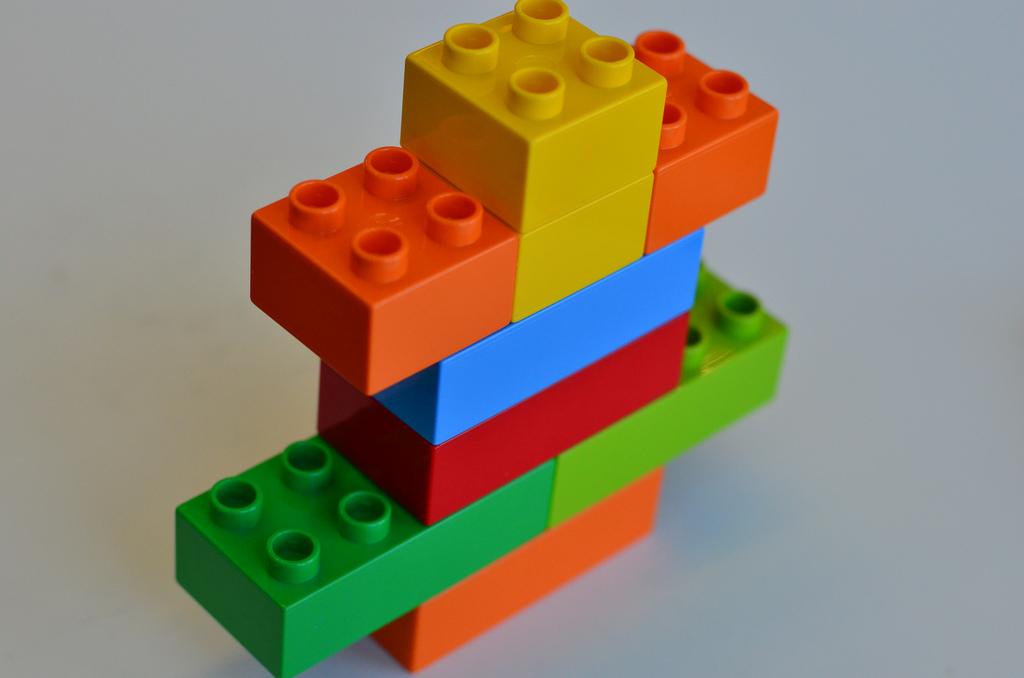
\includegraphics{media/lego.jpg}
\caption{Mattoncini Lego come metafora dei sintagmi}
\end{figure}

Possiamo dividere queste unità, che chiameremo \textbf{costituenti} come sinonimo di sintagma, all'interno di parentesi quadre, così da mostrare i rapporti sintattici:

\begin{enumerate}
\def\labelenumi{(\arabic{enumi})}
\setcounter{enumi}{9}
\item
  \begin{enumerate}
  \def\labelenumii{\alph{enumii}.}
  \tightlist
  \item
    I topi non avevano nipoti.\\
  \item
    {[} I topi {]} {[} non avevano {[} nipoti {]} {]}.
  \end{enumerate}
\end{enumerate}

oppure mostrare l'organizzazione sintattica attraverso un cosiddetto \emph{diagramma ad albero} come nell'esempio seguente:

\begin{figure}

{\centering 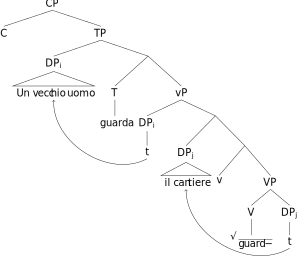
\includegraphics[width=0.7\linewidth]{sintassiIta2_files/figure-latex/tree1-1} 

}

\caption{Rappresentazione ad albero di una frase transitiva}\label{fig:tree1}
\end{figure}

Uno studente attento potrebbe notare qualche differenza rispetto ad una notazione ad albero precedente:

\begin{figure}

{\centering 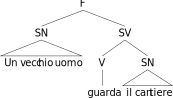
\includegraphics[width=0.7\linewidth]{sintassiIta2_files/figure-latex/tree2-1} 

}

\caption{Rappresentazione secondo lo schema X-barra}\label{fig:tree2}
\end{figure}

La prima e più semplice differenza che possiamo notare è nella denominazione dei costituenti: il primo albero presenta una notazione inglese, mentre il secondo in italiano. Così \emph{Determiner Phrase} (DP) corrisponde grosso modo a SN, mentre il sintagma verbale (SV) si compone di diversi livelli (VP, vP, TP), che corrispondono all'unione della radice verbale V, al sintagma v (che possiamo dire legato alla transitività -ma v è un po' problematico) ed a quello di tempo finito T. C invece è il costituente iniziale, che nelle frasi semplici italiane non è pronunciato (ma vedremo oltre che è presente in altri contesti).
Così, la derivazione procede sulla linea dei costituenti C-T-v-V.

\hypertarget{le-proprieta-della-sintassi}{%
\subsection{Le proprietà della sintassi}\label{le-proprieta-della-sintassi}}

Le differenze tra questi due sistemi di visualizzazioni derivano però da un'importante rivisitazione teorica all'interno della teoria sintattica.

Le proprietà principali della sintassi sono la \textbf{ricorsività} e la \textbf{gerarchia}.
Con il termine \emph{ricorsivo} definiamo quella capacità linguistica di poter aggiungere sempre ulteriore materiale linguistico ad una frase, seguendo certe regole: in pratica possiamo immaginare di poter aggiungere sempre un mattoncino Lego alla costruzione ottenuta dall'unione dei mattoncini.
Definiamo questa proprietà della sintassi come \emph{generativa}, e risulta in un indefinito (virtualmente infinito) meccanismo di formazione di nuove strutture\footnote{La sintassi permette di agire in via infinita, ma altre limitazioni fisiche (per es. la memoria) impediscono di sperimentare tale uso infinito}. Possiamo dire che questo generare continuamente nuovo materiale sia il motore dell'aspetto \emph{creativo} del linguaggio.\\
Questa capacità ricorsiva della sintassi prevede però un'ulteriore effetto: le strutture sintattiche presentano uguali meccanismi di formazione per cui una frase complessa ha la stessa geometria di un singolo costituente. Il minimo e il complesso, in questa descrizione linguistica, condividono le proprietà basilari di formazione.

\begin{figure}
\centering
\includegraphics{media/broccolo.jpg}
\caption{Broccolo romanesco: un esempio di ricorsività in natura}
\end{figure}

Con \emph{gerarchia} invece ci riferiamo a quella proprietà della sintassi, che opera su un piano diverso da quello con cui siamo soliti interagire nella lingua. La nostra esperienza linguistica quotidiana infatti è mono-dimensionale, legata all'ordine delle parole nella frase in un senso lineare. Ma il modo in cui costruiamo le frasi non è legato ad uno spazio ad una dimensione, bensì risiede in uno contraddistinto da più dimensioni, con differenti nozioni di località. Così, per esempio, le lingue non sono legate ad una organizzazione sintattica sulla base dell'ordine delle parole (per es. il soggetto non è \enquote{la parola immediatamente vicina al verbo}) bensì al loro ruolo nella struttura sintattica.

\hypertarget{la-geometria-della-sintassi}{%
\subsubsection{La geometria della sintassi}\label{la-geometria-della-sintassi}}

Abbiamo definito questi piccoli mattoncini della sintassi come \emph{costituenti} e abbiamo fatto riferimento ad una certa nozione di \emph{spazio sintattico}. La domanda che potrebbe sorgere sarebbe a questo punto su come sia costituita la \emph{geometria} della sintassi.

Un costituente è un elemento sintattico costituito primariamente dalla sua \emph{testa}, che ne caratterizza il \emph{tipo}. Abbiamo detto inoltre che i costituenti si aggiungono sempre per via binaria, dal basso verso l'alto dell'albero di derivazione: il costituente a cui il costituente in esame si unisce via merge è detto \emph{complementatore}.
Esistono poi altre due posizioni, dette \emph{specificatori} ed \emph{aggiunti}, che insieme formano l'\emph{angolo} del costituente.

\begin{figure}

{\centering 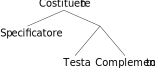
\includegraphics[width=0.7\linewidth]{sintassiIta2_files/figure-latex/tree3-1} 

}

\caption{Raffigurazione di un costituente}\label{fig:tree3}
\end{figure}

Possono essere presenti più specificatori ed ogni specificatore è \emph{equidistante} dalla testa rispetto ad un altro specificatore dello stesso costituente:

\begin{figure}

{\centering 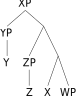
\includegraphics[width=0.7\linewidth]{sintassiIta2_files/figure-latex/tree4-1} 

}

\caption{Un costituente XP}\label{fig:tree4}
\end{figure}

Così, tradizionalmente, alcuni costituenti ospitano 0,1 o più specificatori, che a loro volta possono avere una struttura ramificata: solitamente, in una costruzione finita transitiva in italiano, VP ne ha zero e vP ne ha due.
Ogni costituente presenta 1 testa ed ha uno ed un solo costituente in posizione di complementatore.
Possiamo infatti dire che la testa fornisce l'etichetta del costituente corrispondente (\emph{endocentricità}) e che ogni costituente viene unito ad un altro (l'operazione Merge è binaria), così da avere un solo complementatore.

\begin{figure}

{\centering 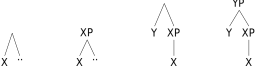
\includegraphics[width=0.9\linewidth]{sintassiIta2_files/figure-latex/tree5-1} 

}

\caption{Una semplice derivazione sintattica}\label{fig:tree5}
\end{figure}

Così le nozioni di \emph{precedenza} e \emph{ordine} risiedono nella struttura sintattica di derivazione, creando una metrica e uno spazio che presenta i propri meccanismi di formazione. Sarà utile infatti tenere a mente che quando parleremo di queste proprietà ci riferiremo primariamente, se non esclusivamente, a tale spazio sintattico.

\hypertarget{i-test-di-costituenza}{%
\subsection{I test di costituenza}\label{i-test-di-costituenza}}

Possiamo definire quali sono i sintagmi di una costruzione linguistica basandoci su alcuni test, che permettono di risolvere qualche incertezza. Prendiamo come esempio la frase:

\begin{enumerate}
\def\labelenumi{(\arabic{enumi})}
\setcounter{enumi}{10}
\tightlist
\item
  Luigi insegna Geologia a Bratislava
\end{enumerate}

Le operazioni che possiamo compiere per catturare i sintagmi della frase sono, per esempio:

\begin{itemize}
\tightlist
\item
  \textbf{Coordinazione}

  \begin{itemize}
  \tightlist
  \item
    Luigi insegna Geologia e Fisica dei Materiali a Bratislava
  \item
    (*) Luigi insegna Geologia e veloce a Bratislava
  \end{itemize}
\item
  \textbf{Ellissi}

  \begin{itemize}
  \tightlist
  \item
    Luigi insegna a Bratislava e anche Maria \emph{(insegna a Bratislava)}
  \end{itemize}
\item
  \textbf{Isolamento}

  \begin{itemize}
  \tightlist
  \item
    A Bratislava \emph{(Dove insegna Luigi?)}
  \item
    Geologia \emph{(Cosa insegna Luigi?)}
  \end{itemize}
\item
  \textbf{Non interruzione}

  \begin{itemize}
  \tightlist
  \item
    (*) a insegna Bratislava Luigi Geologia
  \end{itemize}
\item
  \textbf{Sostituzione} con proforme (p.es. pronome)

  \begin{itemize}
  \tightlist
  \item
    Lui insegna Geologia
  \item
    Lui la insegna lì
  \end{itemize}
\item
  \textbf{Spostamento}

  \begin{itemize}
  \tightlist
  \item
    A Bratislava Luigi insegna Geologia
  \end{itemize}
\end{itemize}

Così, per riprendere la definizione precedente, possiamo pensare alla nozione di \emph{sintagma} come a quella unità sintattica che si compone solitamente di una o più parole, mentre ai \emph{costituenti} come unità che possono anche essere più piccole, arrivando ben al di sotto del livello della parola.

\hypertarget{coordinazione-giustapposizione-subordinazione}{%
\section{Coordinazione, giustapposizione, subordinazione}\label{coordinazione-giustapposizione-subordinazione}}

Se fino a questo momento ci siamo concentrati sulla frase semplice --quella che presenta un predicato verbale e i suoi argomenti-- ora possiamo cominciare ad affrontare il vero nucleo del discorso: la frase complessa ed i modi attraverso cui possiamo unire più frasi tra loro.

Due frasi possono essere unite attraverso una \textbf{coordinazione} (\emph{paratassi}) se si trovano allo stesso livello --vale a dire che possono risultare come frasi a sé:

\begin{enumerate}
\def\labelenumi{(\arabic{enumi})}
\setcounter{enumi}{11}
\tightlist
\item
  Luigi insegna geologia e Maria è una cantante.
\end{enumerate}

Non necessariamente le frasi coordinate sono frasi principali, ma possiamo avere una coordinazione tra strutture di livello secondario ecc:

\begin{enumerate}
\def\labelenumi{(\arabic{enumi})}
\setcounter{enumi}{12}
\tightlist
\item
  Hanno sicuramente molti soldi perché Luigi insegna geologia e Maria è una cantante.
\end{enumerate}

Così, \enquote{\emph{Hanno sicuramente molti soldi}} è la frase \textbf{principale}, mentre \enquote{\emph{perché L.insegna}} è una \textbf{subordinata} della principale e \enquote{\emph{e Maria è una cantante}} è la \textbf{coordinata} della subordinata.

Così, ogni subordinata ha una frase reggente, la quale può essere a sua volta una principale o una subordinata, come in:

\begin{enumerate}
\def\labelenumi{(\arabic{enumi})}
\setcounter{enumi}{13}
\tightlist
\item
  Hanno sicuramente molti soldi perché hanno comprato una casa che hanno pagato moltissimo.
\end{enumerate}

Qui la frase \enquote{\emph{che hanno pagato moltissimo}} continua il discorso della frase reggente \enquote{\emph{hanno comprato una casa}}.
Così la frase reggente non è per forza una principale e in questo esempio abbiamo una principale, una subordinata di 1° grado e una di 2°.

In maniera simile, le costruzioni paratattiche possono essere unite per \textbf{giustapposizione}. In questo caso non vi saranno elementi lessicali ad unirle, bensì segni di punteggiatura:

\begin{enumerate}
\def\labelenumi{(\arabic{enumi})}
\setcounter{enumi}{14}
\tightlist
\item
  Piove. Fa freddo.
\end{enumerate}

\part*{Parte II. \\\ La frase complessa}

\hypertarget{frasi-soggettive}{%
\chapter{Frasi soggettive}\label{frasi-soggettive}}

\hypertarget{funzione}{%
\section{Funzione}\label{funzione}}

\hypertarget{soggettive-esplicite}{%
\section{Soggettive esplicite}\label{soggettive-esplicite}}

\hypertarget{soggettive-implicite}{%
\section{Soggettive implicite}\label{soggettive-implicite}}

\hypertarget{frasi-oggettive}{%
\chapter{Frasi oggettive}\label{frasi-oggettive}}

\hypertarget{funzione-1}{%
\section{Funzione}\label{funzione-1}}

\hypertarget{oggettive-esplicite}{%
\section{Oggettive esplicite}\label{oggettive-esplicite}}

\hypertarget{oggettive-implicite}{%
\section{Oggettive implicite}\label{oggettive-implicite}}

\hypertarget{frasi-interrogative}{%
\chapter{Frasi Interrogative}\label{frasi-interrogative}}

\hypertarget{funzione-2}{%
\section{Funzione}\label{funzione-2}}

\hypertarget{dirette}{%
\section{Dirette}\label{dirette}}

\hypertarget{indirette}{%
\section{Indirette}\label{indirette}}

\hypertarget{esplicite}{%
\section{Esplicite}\label{esplicite}}

\hypertarget{implicite}{%
\section{Implicite}\label{implicite}}

\hypertarget{frasi-relative}{%
\chapter{Frasi Relative}\label{frasi-relative}}

\hypertarget{tipi}{%
\section{Tipi}\label{tipi}}

\hypertarget{esplicite-1}{%
\section{Esplicite}\label{esplicite-1}}

\hypertarget{implicite-1}{%
\section{Implicite}\label{implicite-1}}

\hypertarget{frasi-temporali}{%
\chapter{Frasi temporali}\label{frasi-temporali}}

\hypertarget{definizione}{%
\section{Definizione}\label{definizione}}

\hypertarget{tipi-1}{%
\section{Tipi}\label{tipi-1}}

\hypertarget{esplicite-2}{%
\section{Esplicite}\label{esplicite-2}}

\hypertarget{implicite-2}{%
\section{Implicite}\label{implicite-2}}

\hypertarget{frasi-comparative-e-modali}{%
\chapter{Frasi comparative e modali}\label{frasi-comparative-e-modali}}

\hypertarget{definizione-1}{%
\section{Definizione}\label{definizione-1}}

\hypertarget{tipi-2}{%
\section{Tipi}\label{tipi-2}}

\hypertarget{esplicite-3}{%
\section{Esplicite}\label{esplicite-3}}

\hypertarget{implicite-3}{%
\section{Implicite}\label{implicite-3}}

\hypertarget{frasi-causali-e-finali}{%
\chapter{Frasi causali e finali}\label{frasi-causali-e-finali}}

\hypertarget{definizione-2}{%
\section{Definizione}\label{definizione-2}}

\hypertarget{esplicite-4}{%
\section{Esplicite}\label{esplicite-4}}

\hypertarget{implicite-4}{%
\section{Implicite}\label{implicite-4}}

\hypertarget{frasi-consecutive-e-concessive}{%
\chapter{Frasi consecutive e concessive}\label{frasi-consecutive-e-concessive}}

\hypertarget{definizione-3}{%
\section{Definizione}\label{definizione-3}}

\hypertarget{esplicite-5}{%
\section{Esplicite}\label{esplicite-5}}

\hypertarget{implicite-5}{%
\section{Implicite}\label{implicite-5}}

\hypertarget{frasi-condizionali}{%
\chapter{Frasi condizionali}\label{frasi-condizionali}}

\hypertarget{definizione-4}{%
\section{Definizione}\label{definizione-4}}

\hypertarget{esplicite-6}{%
\section{Esplicite}\label{esplicite-6}}

\hypertarget{implicite-6}{%
\section{Implicite}\label{implicite-6}}

\hypertarget{discorso-diretto-e-indiretto}{%
\chapter{Discorso diretto e indiretto}\label{discorso-diretto-e-indiretto}}

\hypertarget{definizione-5}{%
\section{Definizione}\label{definizione-5}}

\hypertarget{esplicite-7}{%
\section{Esplicite}\label{esplicite-7}}

\hypertarget{implicite-7}{%
\section{Implicite}\label{implicite-7}}

\bibliography{bibliography.bib}

\end{document}
